\documentclass[notes=show notes]{beamer}
%%%%%%%%%%%%%%%%%%%%%%%%%%%%%%%%%%%%%%%%%%%%%%%%%%%%%%%%%%%%%%%%%%%%%%%%%%%%%%%%%%%%%%%%%%%%%%%%%%%%%%%%%%%%%%%%%%%%%%%%%%%%%%%%%%%%%%%%%%%%%%%%%%%%\usepackage{amssymb}
% Sjekk ut
% Eksempel på TARGET-balansen
\usepackage{mathpazo}
\usepackage{hyperref}
\usepackage{multimedia}
\usepackage{graphicx}
\usepackage{amssymb}
%%\usepackage[utf8]{inputenc}
%\usecolortheme[named=black]{structure}
%\usetheme[height=10mm]{Rochester}
\usetheme{Dresden}
%\input{tcilatex}
\begin{document}
\author[]{J\o rn Inge Halvorsen }
\title[]{Krisen i Eurosonen og TARGET-ubalanser}
\date[]{7. november, 2014}
\institute[J\o rn Inge Halvorsen]{Forelesning for Universitetet i Agder}
\maketitle	
\begin{frame}{Lange renter p\aa \  10-\aa rige statsobligasjoner}
\begin{figure}
\centering
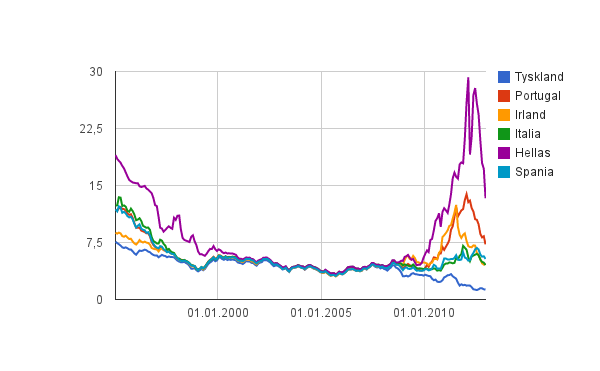
\includegraphics[width=0.9\linewidth]{Fig2_Lange_Renter_G}
%\center Kilde: Eurostat
%\caption{}
\label{fig:Fig2_Lange_Renter_G}
\end{figure}
\end{frame}
\begin{frame}{Relative utviklingen i BNP deflatoren i forhold til Tyskland}
\begin{figure}
\centering
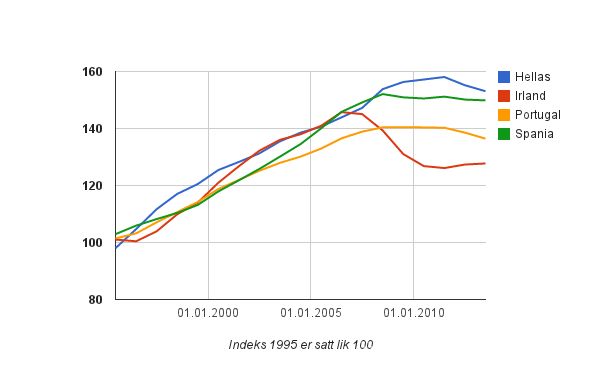
\includegraphics[width=0.80\linewidth]{Fig3_bnp_deflator_g}
%\caption{}
\begin{itemize}
\item Estimert behov for intern devaluering:
%\footnote[]{Goldman Sachs European Economic Analysis (2013)}\\ 
\begin{itemize}
	\item Portugal, Spania, Irland: 25-35 prosent. 
	\item Irland 0 prosent. 
\end{itemize} 
\end{itemize}
\label{fig:Fig3_bnp_deflator_g}
\end{figure}
\end{frame}	
\begin{frame}{TARGET-balansen til de nasjonale sentralbankene}
%(+) TARGET-fordringer, (-) TARGET-gjeld
\begin{figure}
\centering
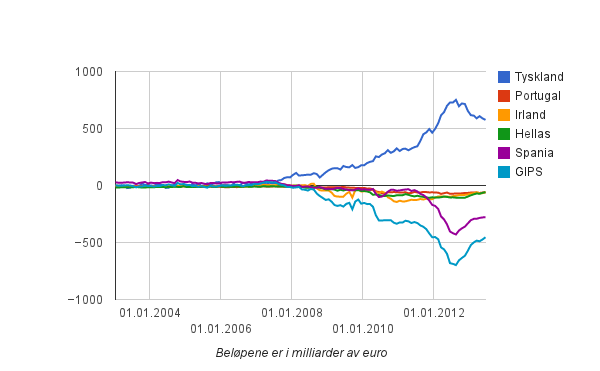
\includegraphics[width=0.9\linewidth]{Fig4_TARGET_gjeld_fordringer_G}
\center \small{Kilde: Datastream, basert p\aa \   Sinn \& Wollmershauser (2012)}
%\caption{}
\label{fig:Fig4_TARGET_gjeld_fordringer_G}
\end{figure}
\end{frame}
\begin{frame}{Forklaring 1: TARGET-ubalanser for\aa rsaket av 
		\o kte reserver}
\begin{figure}
\centering
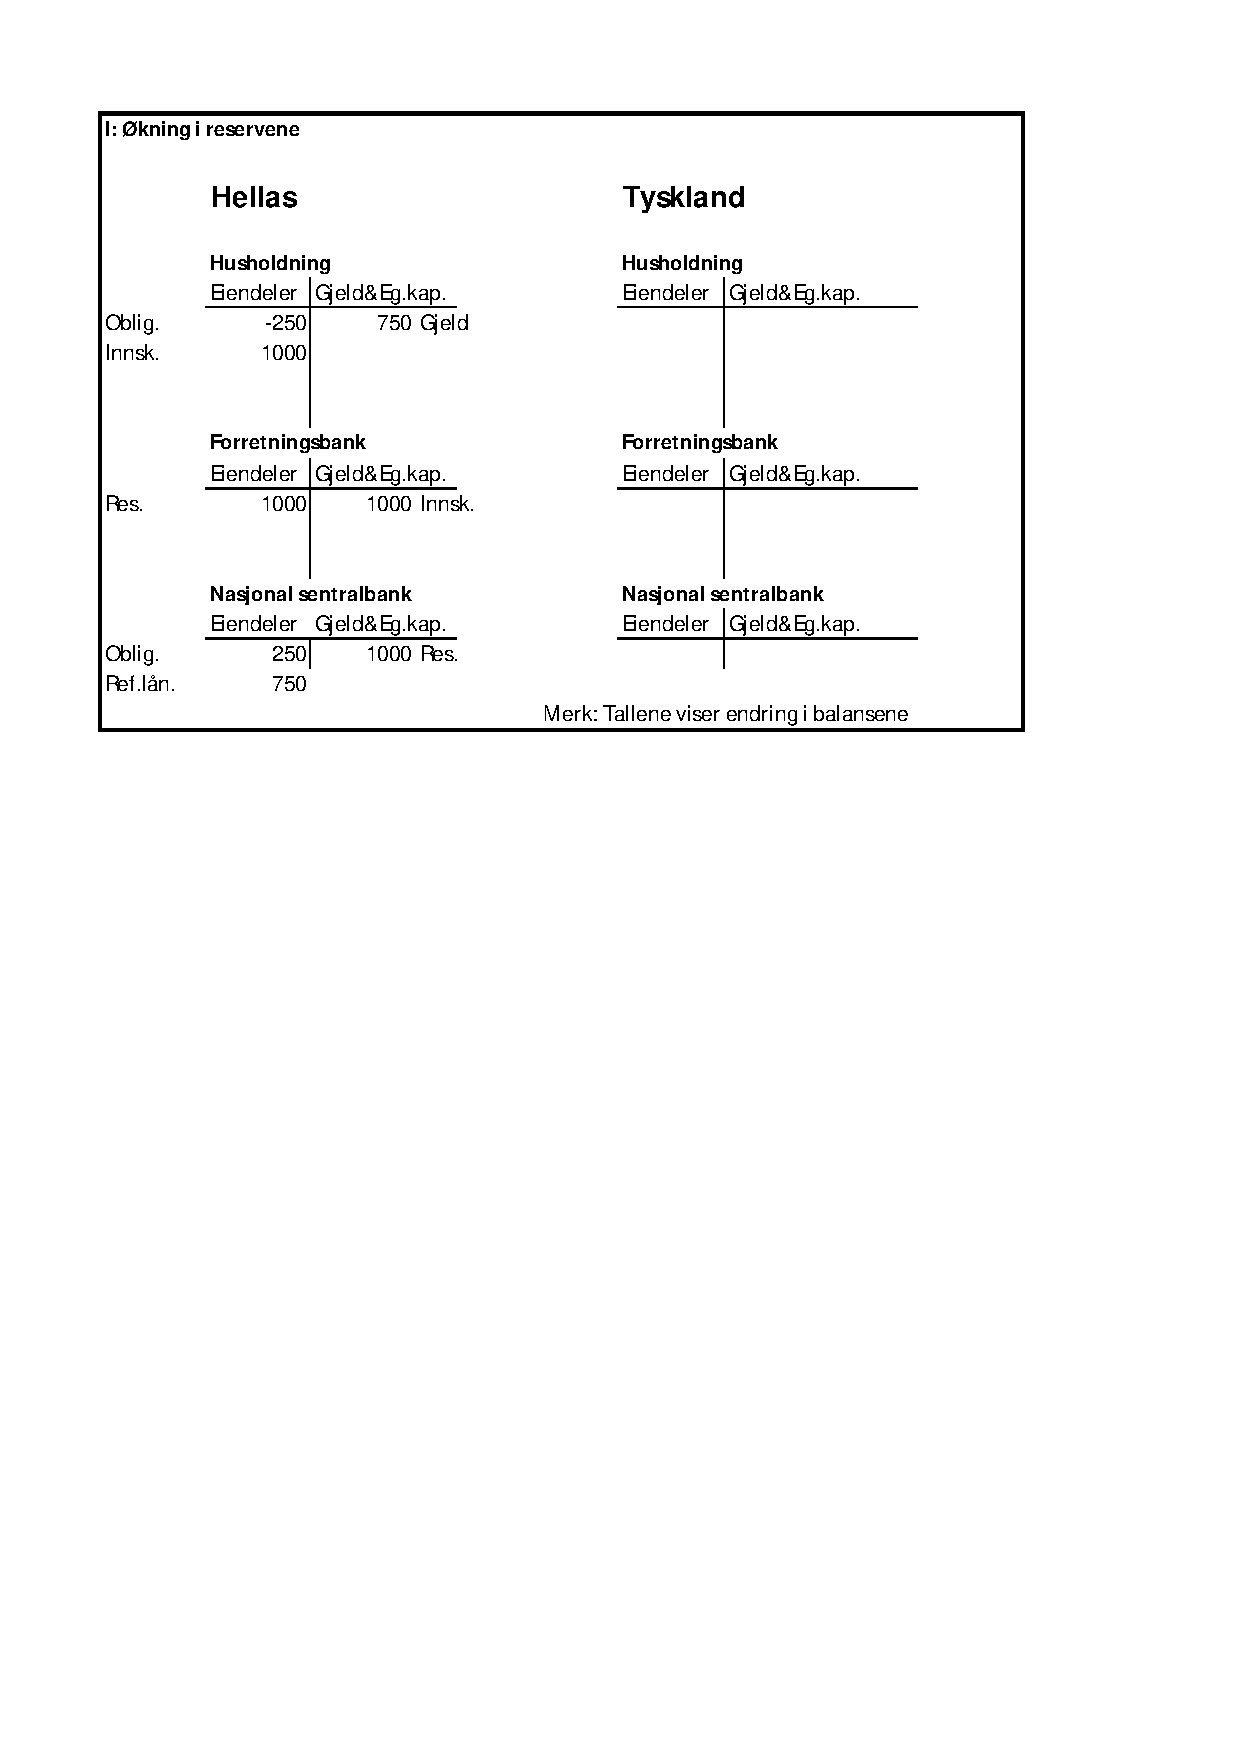
\includegraphics[width=0.9\linewidth]{Fork1_delI}
\label{fig:Fork1_dellI-1}
\end{figure}
\end{frame}
\begin{frame}
\begin{figure}
\centering
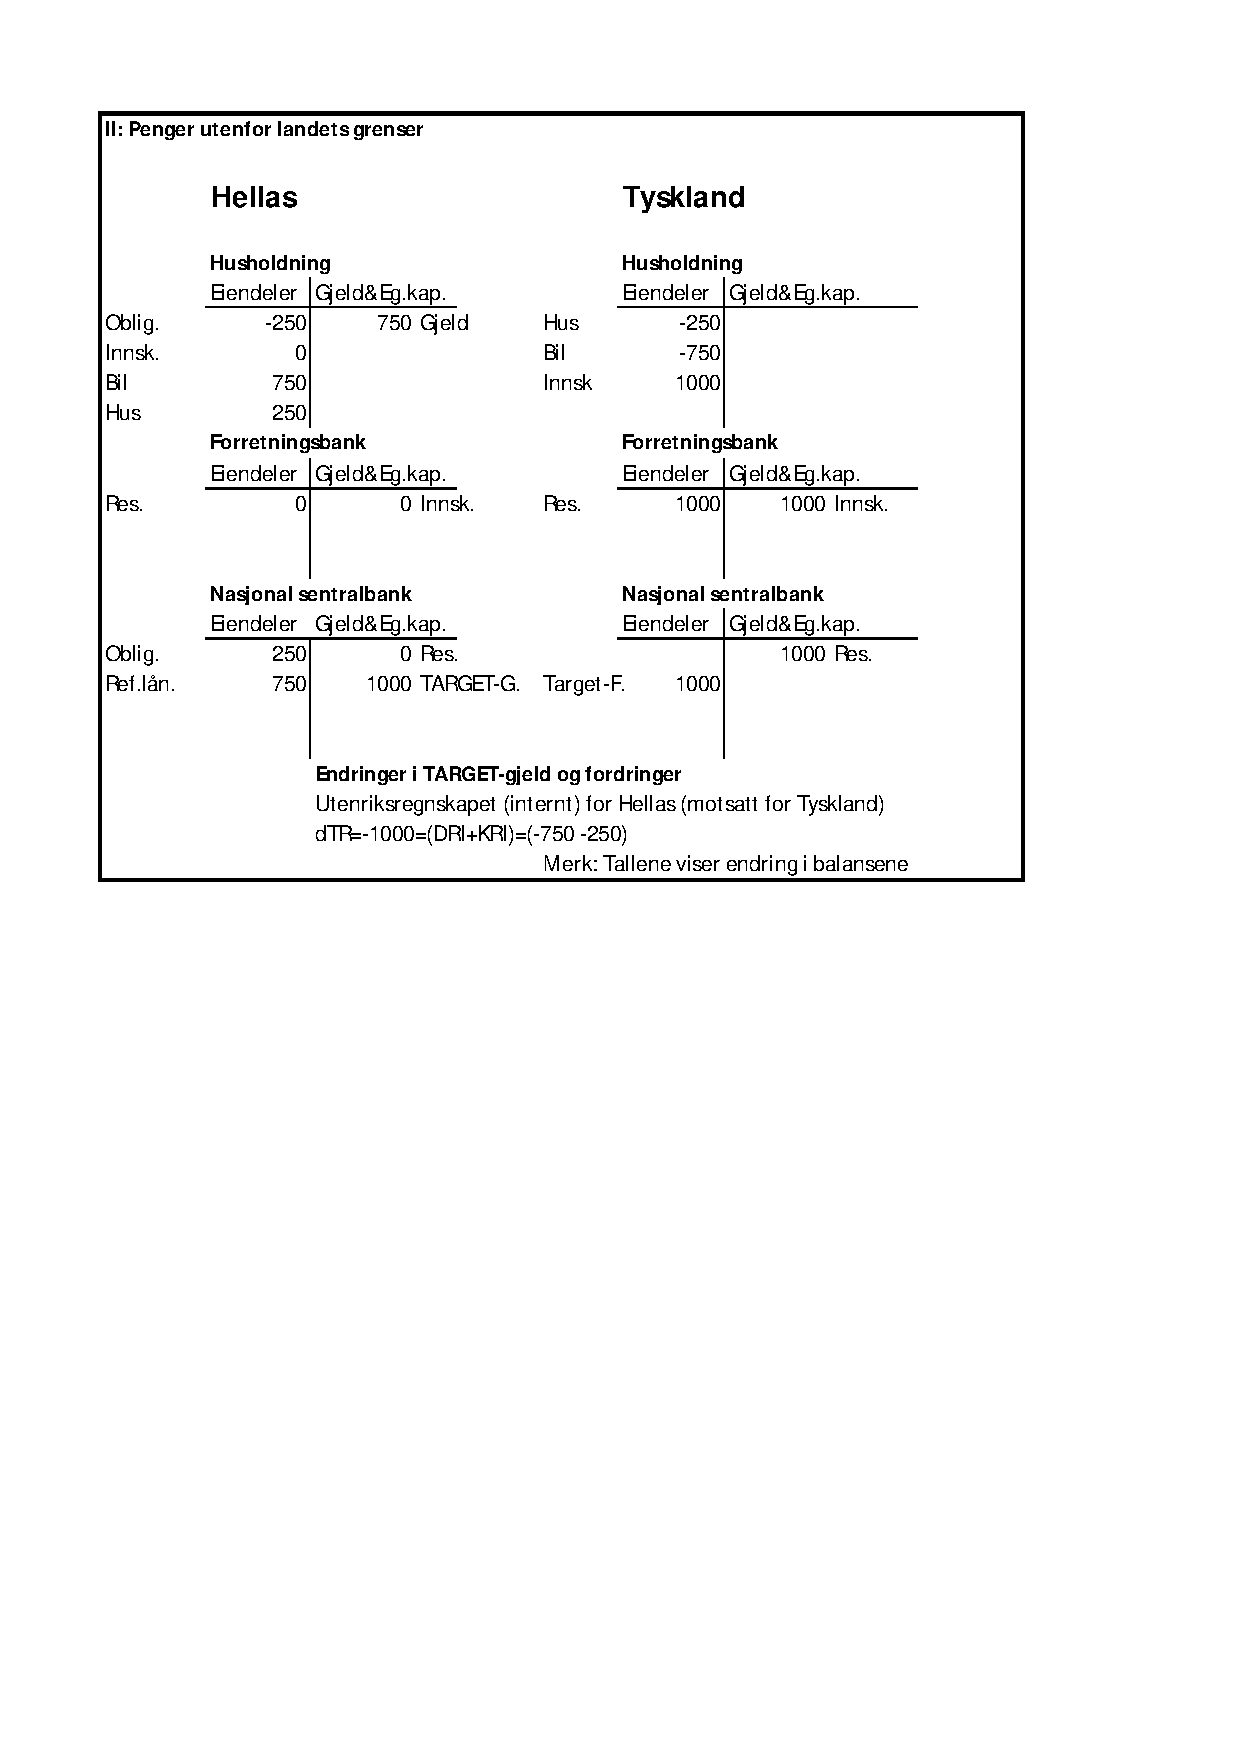
\includegraphics[width=0.9\linewidth]{Fork1_delII}
\caption{}
\label{fig:Fork1_delII}
\end{figure}
\end{frame}
\begin{frame}{Forklaring 2: TARGET-ubalanser for\aa rsaket av kapitalflukt}
\begin{figure}
\centering
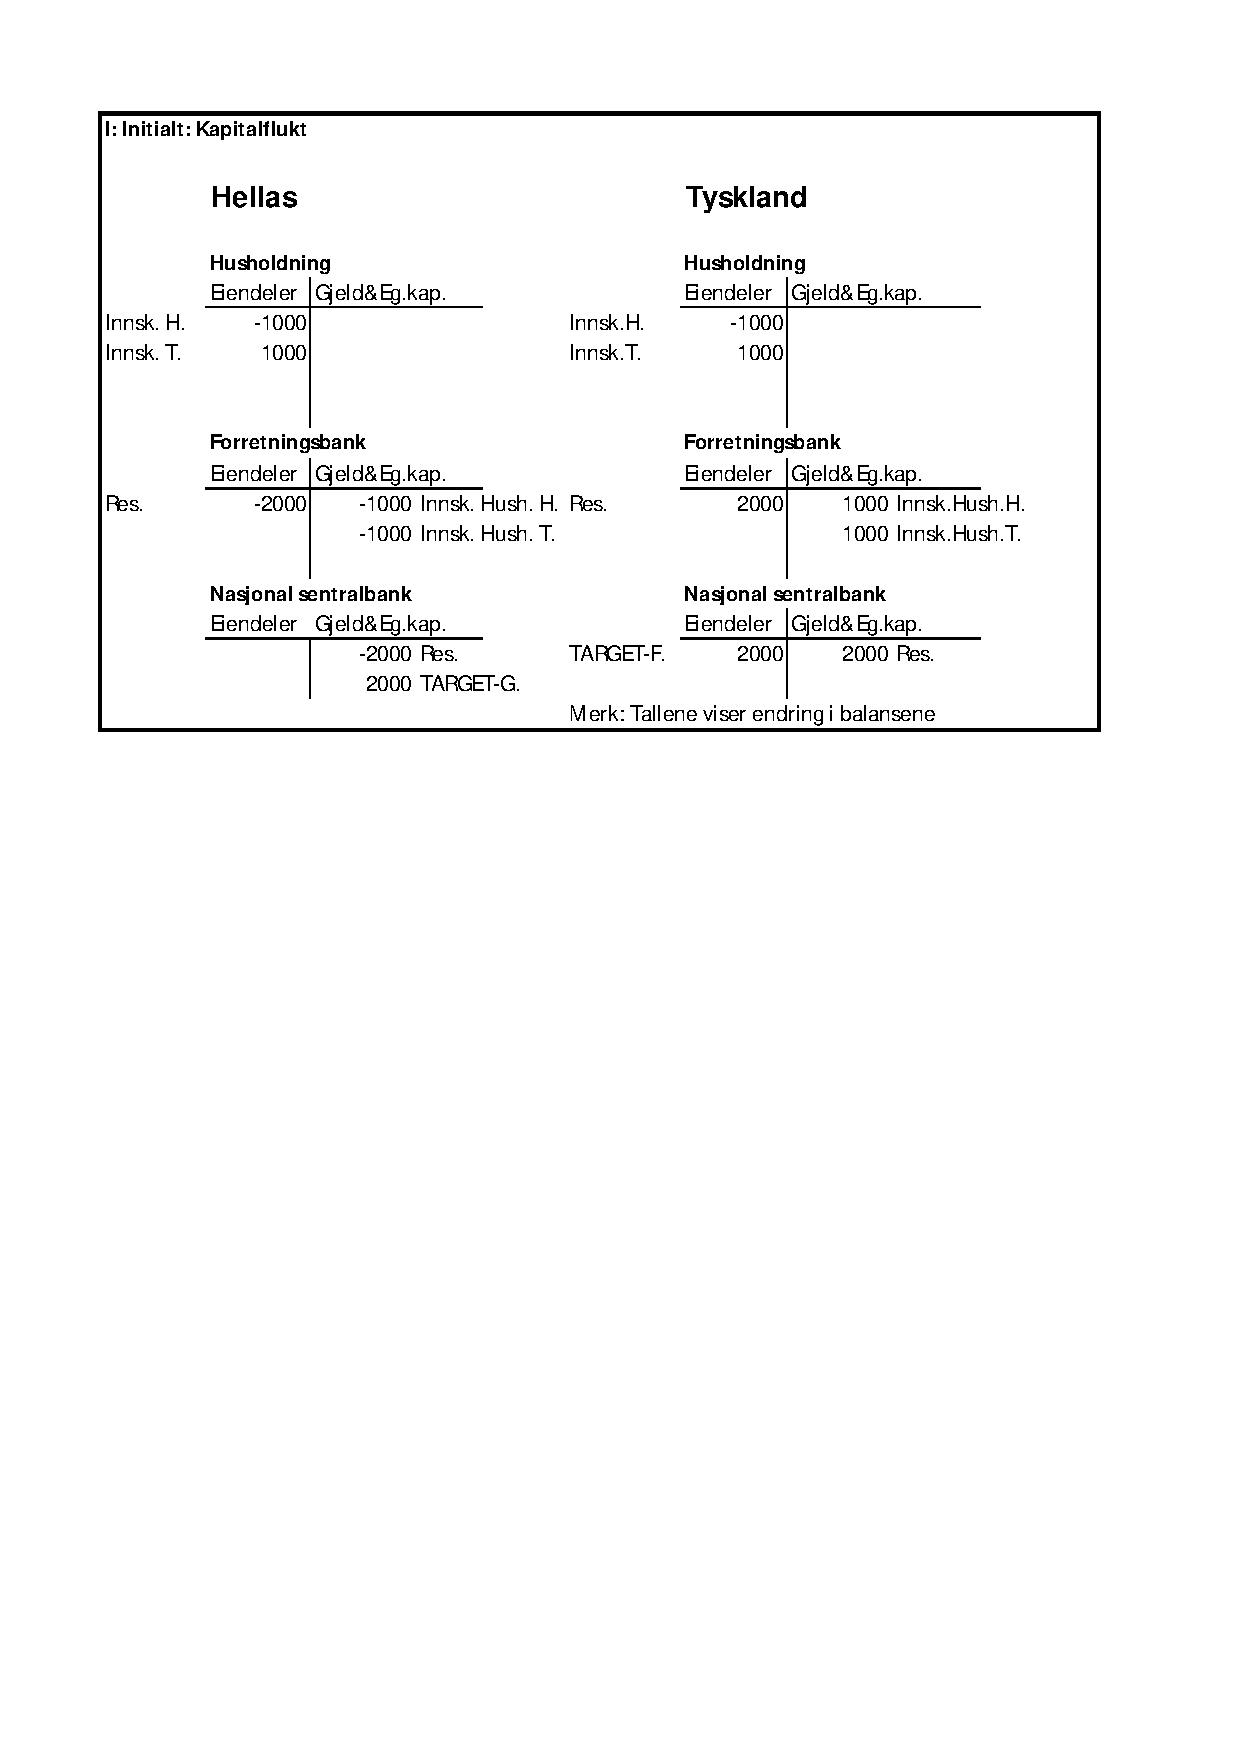
\includegraphics[width=0.9\linewidth]{Fork2_delI}
\label{fig:Fork1_delII}
\end{figure}
\end{frame}
\begin{frame}
\centering
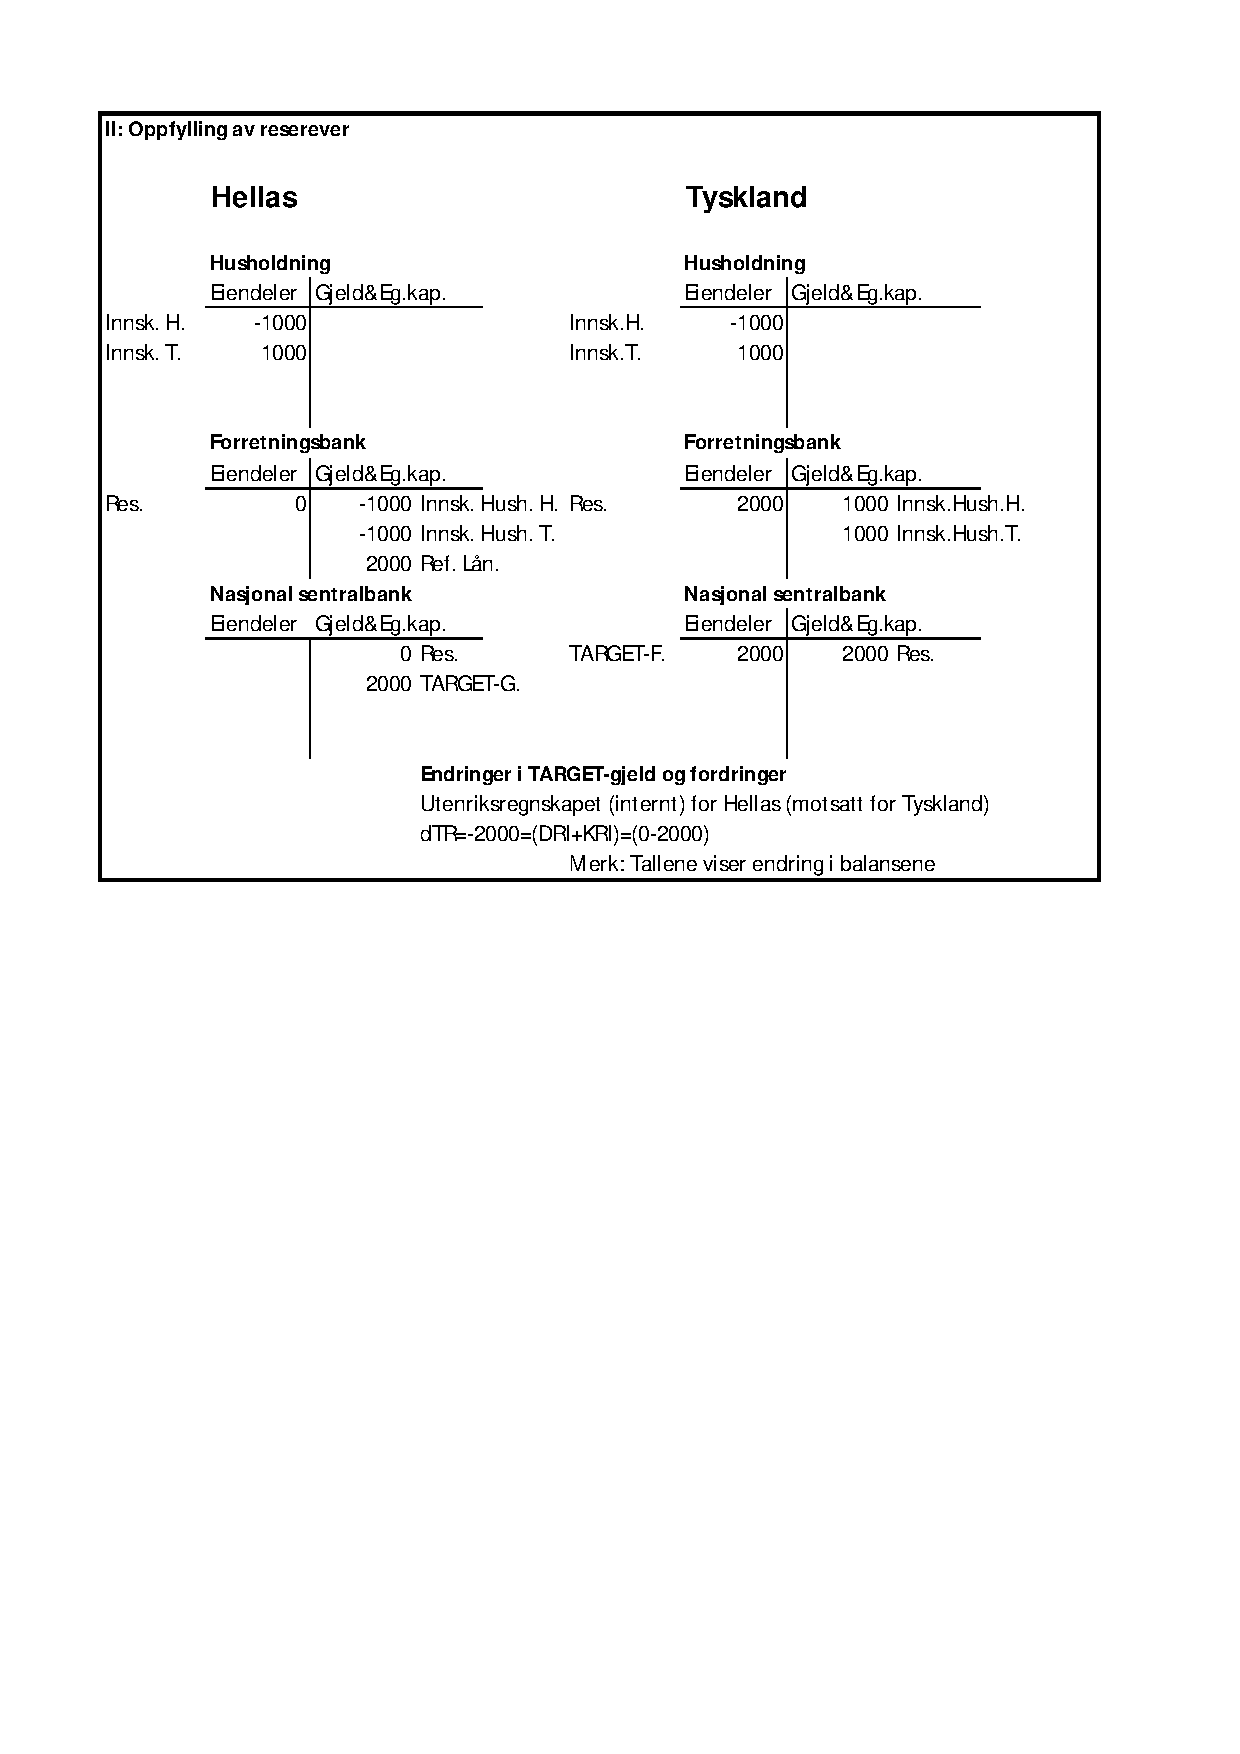
\includegraphics[width=0.8\linewidth]{Fork2_delII}
\end{frame}
\begin{frame}{Hvorfor vil asymmetrisk vekst basispengemengden kunne oppst\aa ?}
\begin{itemize}
\item Forretningsbankene i Eurosonen kan velge mellom to former for finansiering: 
\begin{enumerate}
\item Refinansieringsl\aa n -- renta skal v\ae re lik for alle forretningsbankene i Eurosonen.
\item Markedsfinansiering (eks. interbank) --  renta avhenger av markedsakt\o renes oppfatninger om bankens soliditet.
\end{enumerate}
\item Dersom greske banken anses som mindre solid enn den tyske, vil kostnadsminimering kunne bety at den greske velger refinansieringsl\aa n og den tyske markedsfinansiering. 
\end{itemize}
\end{frame}
\begin{frame}{Kontrafaktisk analayse: Hva ville ha skjedd dersom ESB \o nsket \aa \ holde basispengemengden uendret?}
\begin{itemize}
\item ESB kunne ha oppn\aa dd dette ved hevet krav til sikkerhet og \o kt rente.
\item Forklaring 1:\\
	$\uparrow i=\text{i}_{m} \Rightarrow \text{C og I}\downarrow \Rightarrow \text{Y}\downarrow \Rightarrow P\downarrow ...$
\item Forklaring 2:\\
$\uparrow i=\text{i}_{m} \Rightarrow \Delta\text{TG}=0 \footnote{Ved markedssvikt kan vi her f\aa \ et l\o p p\aa \ bankene.} \Rightarrow, \text{C og I}\downarrow \Rightarrow \text{Y}\downarrow \Rightarrow P\downarrow ...$
%\item $NX(R,Y,Y^{*})=X(R,Y^{*})-R\cdot IM(R,Y)$
\item N\aa r $Y\downarrow$ og $P \downarrow$, vil driftsbalansen bedres som et resultat av \o kt nettoeksport.  
\end{itemize}
\end{frame}	
\begin{frame}{ESBs pengepolitikk i etterkant av finanskrisen}
\begin{itemize}
\item Fra oktober 2008 til mai 2010 ble renta p\aa\  refinansieringsl\aa n redusert fra 4,25 til 1 prosent.
\item Kravet til sikkerhet ble samtidig senket fra A- til BBB-.
\item Ytterligere reduksjon i sommeren 2010: ELA l\aa n (uten krav til sikkerhet)
\end{itemize}
\end{frame}	
\begin{frame}{Utviklingen i driftsbalansen og TARGET-gjelden for PIGS-landene i etterkant av finanskrisen}
	\begin{figure}
\centering
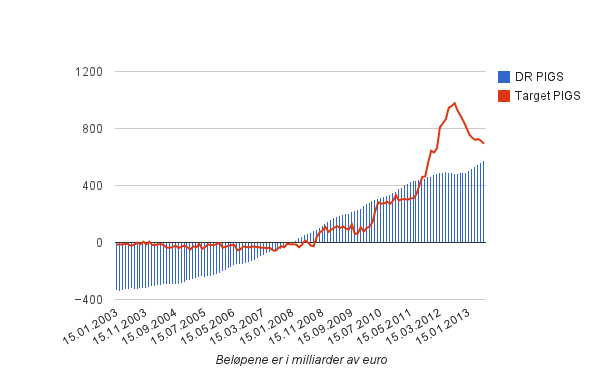
\includegraphics[width=0.8\linewidth]{Fig7_TARGET_Driftsbalanse_G}
\label{fig:Fig7_TARGET_Driftsbalanse_G}
\center \small{Kilde: Datastream, basert p\aa \   Sinn \& Wollmershauser (2012)}
\end{figure}
\end{frame}	
\begin{frame}
	\textbf{Resultat 1: ESB har ved sin pengepolitikk satt til side de selvkorrigerende mekanismene som gjelder for driftsbalansen mellom land i Eurosonen.}
\end{frame}
\begin{frame}{Fordelingseffekter av ESBs pengepolitikk}
\begin{itemize}
	\item Overskuddet til ESB (seigniorage) er gitt ved inntektene fra aktive-siden fratrukket forpliktelsen for gjeld fra passiva-siden.
	\item Siden rentekostnaden for TARGET-gjeld er lik rentinntektene for TARGET-fordringer, nettes disse postene mot hverandre n\aa r en betrakter systemet som helhet.
\end{itemize}
\end{frame}	
\begin{frame}{Endring i balansepostene tilknyttet forklaring 1}
\begin{figure}
\centering
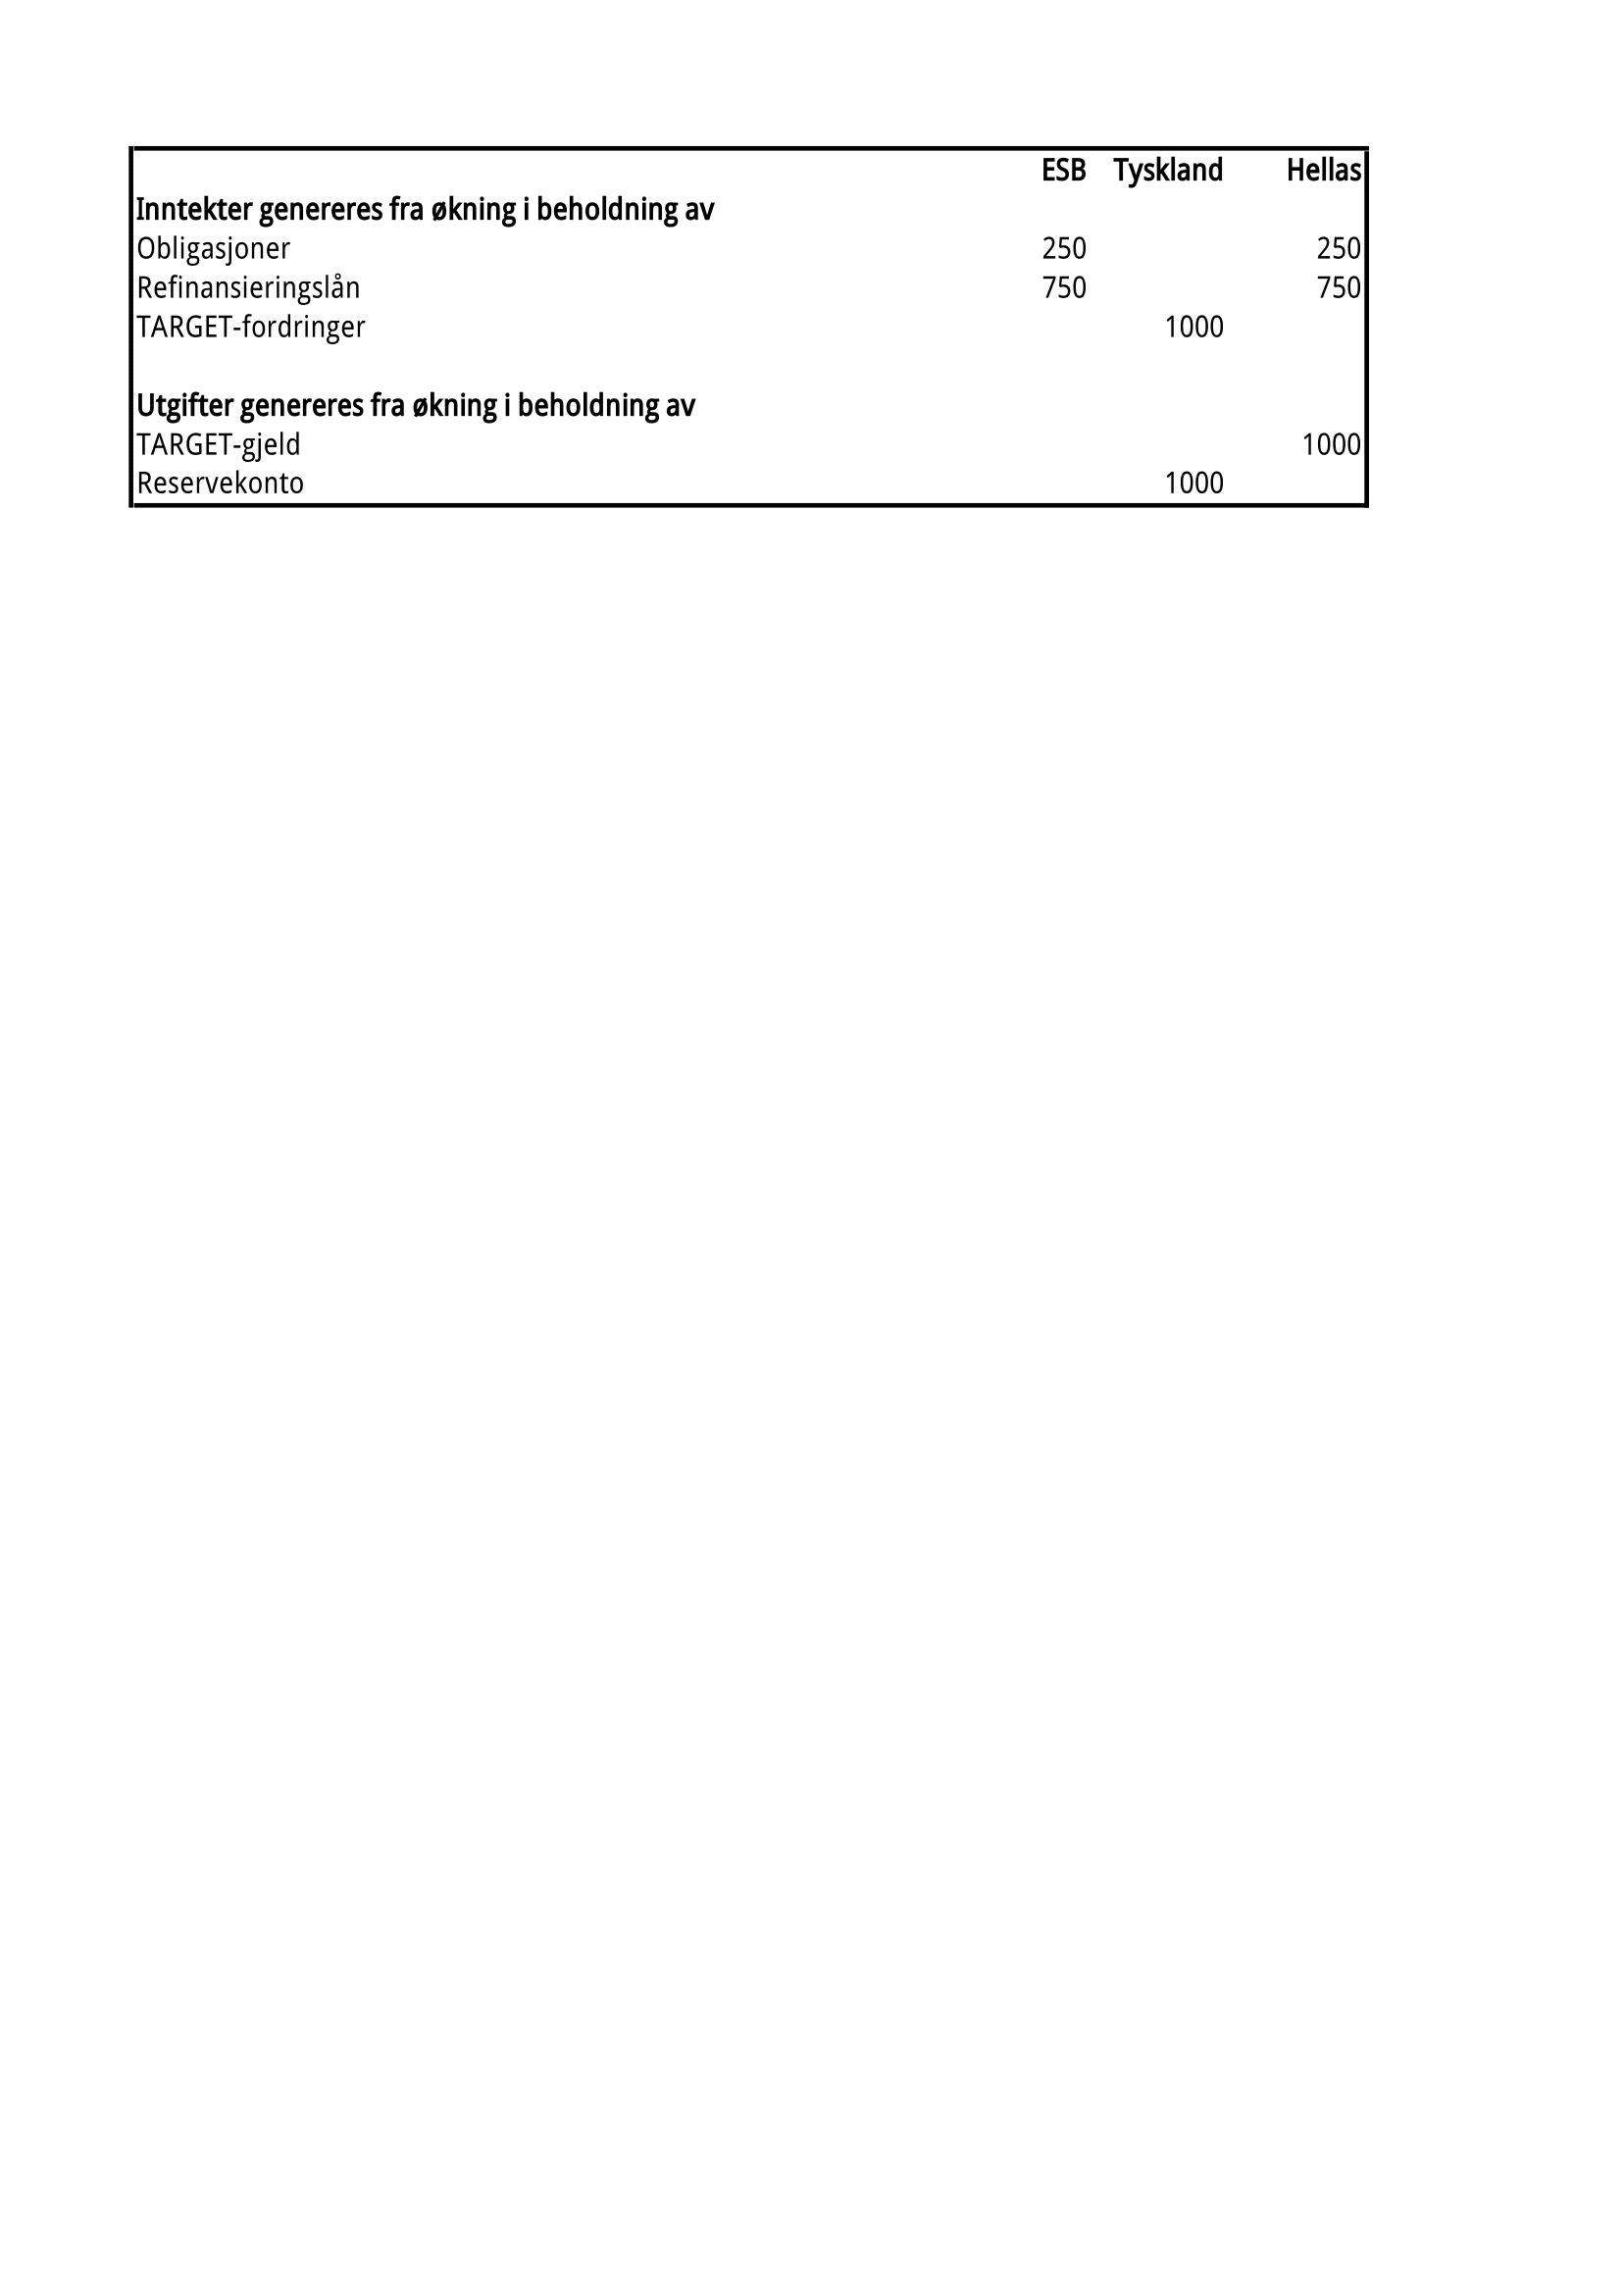
\includegraphics[width=0.9\linewidth]{SenFork1-1}
\caption{}
\label{fig:SenFork1-1}
\end{figure}
\end{frame}	
\begin{frame}{Endring i balansepostene tilknyttet forklaring 2}
\begin{figure}
\centering
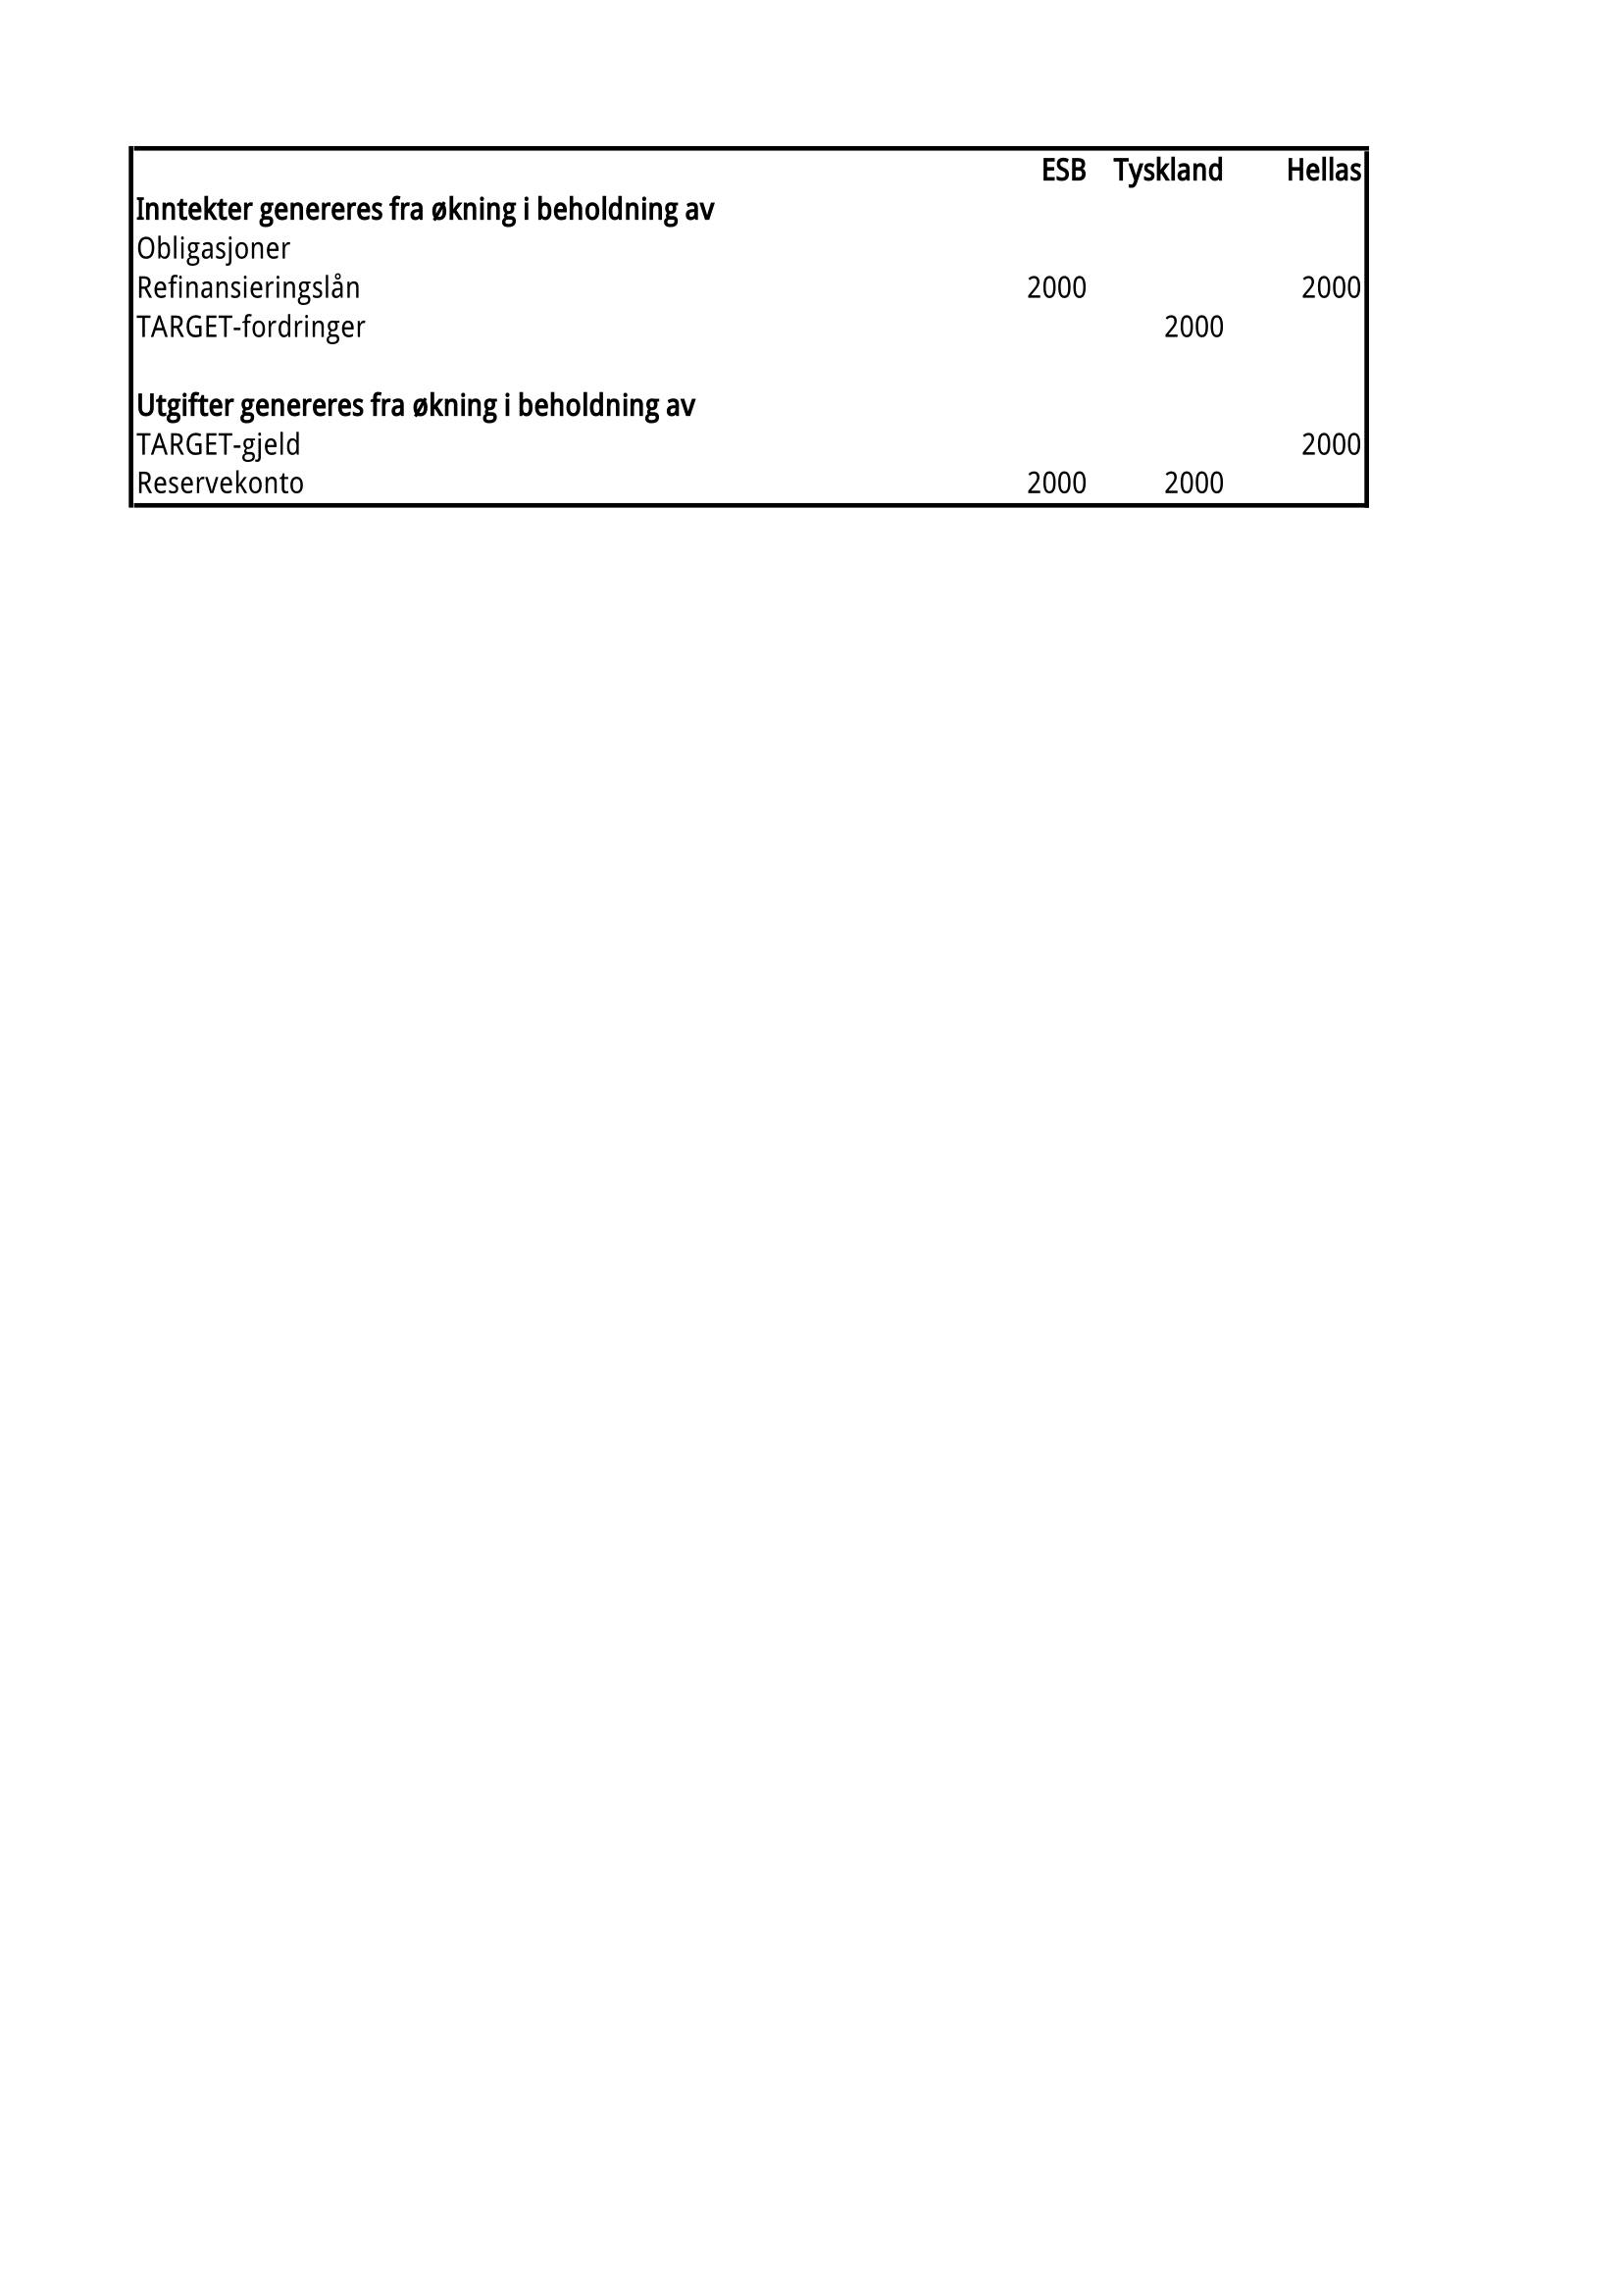
\includegraphics[width=0.9\linewidth]{SenFork2-1}
\caption{}
\label{fig:SenFork2}
\end{figure}
\end{frame}	
\begin{frame}
\begin{itemize}
\item Overf\o ringen av risiko til nasjonale skattebetalere skjer fordi ESB alternativt kunne benyttet de samme reservene til en sikrere plassering.
\end{itemize}	
\end{frame}			
\begin{frame}
\textbf{Resultat 2: ESB krisepolitikk har i storstilt grad overf\o rt risiko fra internasjonale finansinvestorer til nasjonale skattebetalere.}
\end{frame}			
%	\item Overføringen av risiko til nasjonale skattebetalere skjer fordi ESB alternativt kunne benyttet de samme reservene til en sikrere pengeplassering. 
%	\item Dette betyr inneb\ae rer en lavere utbetalinger til nasjonale myndigheter n\aar en d\aa %rlig tilstand f\o rst inntreffer. 
%	\item Dersom gjeldsniv\a et skal v\ae re det samme, 
\begin{frame}{Rasjonelle forventninger og eliminering av rentespreaden}
	\begin{enumerate}
		\item Legger vi til grunn at internasjonale finansinvestorer tidligere har vurdert  
		ESBs realiserte politikkrespons som sv\ae rt sannsynlig.
		\item En f\o lge ville i s\aa \ fall ha v\ae rt et redusert behov for kontroll av usikkerheten til motagerne av de l\aa nte pengene. 
		\item Med det resultat at l\aa neivrige l\aa netakere i stor grad har v\ae rt de som har blitt prioritert f\o rst.
	\end{enumerate}
\end{frame}
\begin{frame}
\textbf{Resultat 3: Rasjonelle forventninger knyttet til den politikken som har blitt realisert gir en  \o konomisk forklaring p\aa \ hvorfor rentespreaden ble eliminert ved innf\o ringen av euroen.}
\end{frame}
\begin{frame}{Veien videre?}
Til slutt la oss see p\aa \ tre ulike politikkveivalg for Eurosonen og vurdere dets p\aa virkning p\aa  \ intern og ekstern balanse samt finansiell stabilitet.
\end{frame}
\begin{frame}{Alternativ 1: Tilbake til markedene}
\begin{itemize}
	\item Stramme inn kravene til sikkerhet p\aa \ refinansieringsl\aa n  slik at forretningsbankene
	prim\ae rt finansierer seg gjennom markedet.
\end{itemize}
Igangsette prosessen mot intern- og ekstern balanse, men med \o kt fare for finansiell ustabilitet.
\end{frame}
\begin{frame}{Alternativ 2: \O kt inflasjon i nord}
\begin{itemize}
	\item Markedsfinansiering, nullrente, gjeldsslette og ekpansiv finanspolitikk for landene i nord.
\end{itemize}
Som under alternativ 1, men med \o kt hastighet og redusert sannsynlighet for finansiell ustabilitet.
\end{frame}
\begin{frame}{Alternativ 3: ESM, OMT, bankunion og euroobligasjoner}
\begin{itemize}
	\item Reduserer rentespreaden. 
\end{itemize}
Trolig sikre finansiell stabilitet, men n\ae rmest stanse opp prosessen mot intern og ekstern balanse.
\end{frame}
\end{document}